\documentclass{article}

\usepackage[main=english,vietnamese]{babel}
\usepackage[T1]{fontenc}
\usepackage[utf8]{inputenc}
\usepackage[sexy]{evan}
\usepackage{matchsticks}
\usepackage{wrapfig}
\usepackage{listings}

\title{A simple geometry problem}
\author{Nghia Doan}
\date{\today}

\begin{document}

\maketitle

Usually approaching a problem from different angles help to see different nature of the problem,
more importantly of what we learned, and how to apply them.
In this article, we shows five different approaches, or solutions, to a simple geometry problem.

\begin{example*}
    
    $ABCD$ is a square. $E$ is the midpoint of side $AD,$
    and $F$ is the foot of the altitude from $C$ to $BE.$
    Prove that $DF = DA.$
\end{example*}

\begin{figure}[h]
    \centering
    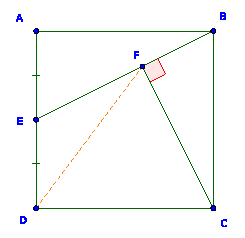
\includegraphics[width=5cm]{./svg/pdf/2022-2-ms-1-1.pdf}
\end{figure}

\begin{proof}[First proof - Using congruent triangles]
    Extending $FE$ to intersect $CD$ at $G,$ see the diagram on the left. 
    Since $\angle AEB = \angle GED, AE = ED, \angle EAB = \angle EDA = 90\dg,$
    by the angle-side-angle (ASA) rule, $\triangle EAB \cong \triangle EDG,$
    thus the corresponding pair of sides are the same, or $DG=AB$. Therefore $DG=DC.$

    \begin{figure}[h]
        \centering
        \begin{minipage}[t]{8cm}
            \centering
            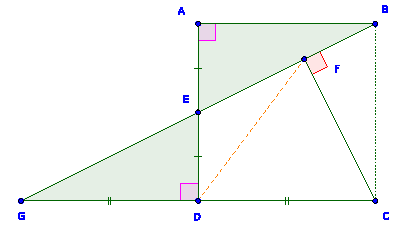
\includegraphics[width=8cm]{./svg/pdf/2022-2-ms-1-1-a.pdf}
        \end{minipage}
        \quad
        \begin{minipage}[t]{8cm}
            \centering
            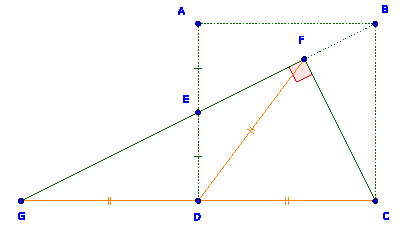
\includegraphics[width=8cm]{./svg/pdf/2022-2-ms-1-1-b.pdf}
        \end{minipage}
    \end{figure}

    Now, it is a well-known fact that,
    \textit{the midpoint of the hypotenuse of a right triangle is at equidistance from all vertices.}
    Using this fact for $\triangle DGC$ in the diagram on the right in the figure above,
    $DG=DC,\ \angle{GFC} = 90^\circ,$ thus $DF=DG=DC.$
\end{proof}

\newpage

\begin{proof}[Second proof - Using median segment]
    Let $G$ be the midpoint of $BC,$ and let $DG$ intersect $FC$ at $H.$
    By side-side-side (SSS) $\triangle EAB \cong \triangle GCD,$
    so $\angle ABE = \angle CDG \Rightarrow EB \parallel DG.$

    \begin{figure}[h]
        \centering
        \begin{minipage}[t]{8cm}
            \centering
            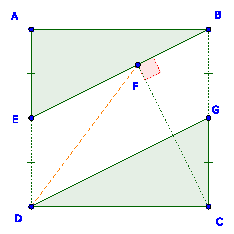
\includegraphics[width=5cm]{./svg/pdf/2022-2-ms-1-1-c.pdf}
        \end{minipage}
        \quad
        \begin{minipage}[t]{8cm}
            \centering
            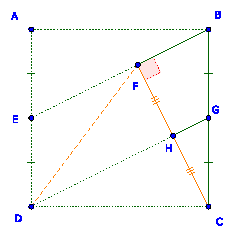
\includegraphics[width=5cm]{./svg/pdf/2022-2-ms-1-1-d.pdf}
        \end{minipage}
    \end{figure}

    Furthermore, in $\triangle FBC,$ $GH \parallel BF,$ $G$ is midpoint of $BC,$
    so $H$ is midpoint of $FC.$
    Finally, in $\triangle DFC,$ $DH \perp FC,$ $H$ is midpoint of $FC,$
    thus by side-angle-side (SAS) $\triangle DHF \cong \triangle DHC,$ hence $DF = DC.$

    \begin{figure}[h]
        \centering
        \begin{minipage}[t]{8cm}
            \centering
            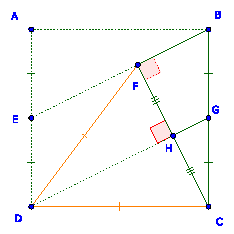
\includegraphics[width=5cm]{./svg/pdf/2022-2-ms-1-1-e.pdf}
        \end{minipage}
    \end{figure}
\end{proof}

\begin{proof}[Third proof - Using angles in circle]
    Both $\triangle EDC$ and $\triangle EFC$ are right at $D$ and $F.$
    $C, D, E,$ and $F$ are on the circle centred at $G.$

    \begin{figure}[h]
        \centering
        \begin{minipage}[t]{8cm}
            \centering
            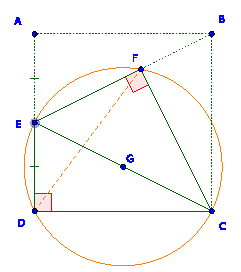
\includegraphics[width=5cm]{./svg/pdf/2022-2-ms-1-1-f.pdf}
        \end{minipage}
        \quad
        \begin{minipage}[t]{8cm}
            \centering
            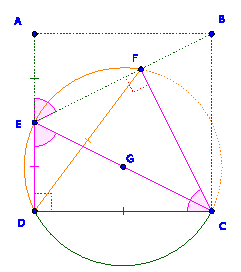
\includegraphics[width=5cm]{./svg/pdf/2022-2-ms-1-1-g.pdf}
        \end{minipage}
    \end{figure}

    $\angle DEC = \angle AEB = 180^{\circ} - \angle DEF = \angle DCF.$ 
    $\angle DEC = \angle DFC$ (subtends arc $DC$).
    $\angle DCF = \angle DFC$, $\triangle DCF$ is isosceles, thus $DC = DF.$
\end{proof}

\newpage

\begin{proof}[Fourth proof - Using triangle trigonometry]
    First, by Pythagorean theorem, $EB = \sqrt{AB^2 +AE^2} = \frac{a\sqrt{5}}{2}.$
    Then, let $\alpha = \angle DCF = \angle FBC = \angle AEB.$
    It is easy to see that $\cos{\alpha} = \frac{AE}{EB} = \frac{1}{\sqrt{5}},$
    and since $\triangle FCB \sim \triangle ABE$, $\frac{FC}{BC} = \sin{\alpha} = \frac{AB}{EB} = \frac{2}{\sqrt{5}},$
    so $FC = BC \sin{\alpha} = \frac{2a}{\sqrt{5}}.$

    \begin{figure}[h]
        \centering
        \begin{minipage}[t]{8cm}
            \centering
            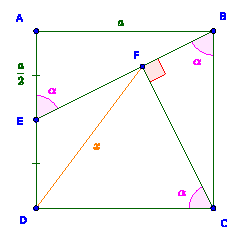
\includegraphics[width=5.5cm]{./svg/pdf/2022-2-ms-1-1-h.pdf}
        \end{minipage}
    \end{figure}

    By the Law of Cosines,
    $DF = \sqrt{DC^2 +  FC^2 - 2(DC)(FC)\cos{\alpha}}
    = \sqrt{a^2 + \left(\frac{2a}{\sqrt{5}}\right)^2 - 2a \frac{2a}{\sqrt{5}} \frac{1}{\sqrt{5}}} = a.$
\end{proof}

\begin{proof}[Fifth proof - Using Ptolemy theorem]
    Similar to the previous proof,
    let $DC = a \Rightarrow EB = EC = \frac{a\sqrt{5}}{2}.$ 
    $\frac{FC}{BC} = \frac{AB}{EB} \Rightarrow FC=\frac{2a}{\sqrt{5}}.$
    $\frac{FB}{BC} = \frac{AE}{EB} \Rightarrow FB=\frac{a}{\sqrt{5}}.$

    \begin{figure}[h]
        \centering
        \begin{minipage}[t]{8cm}
            \centering
            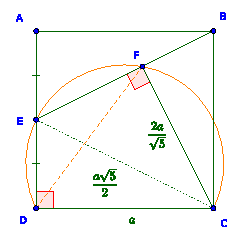
\includegraphics[width=5.5cm]{./svg/pdf/2022-2-ms-1-1-i.pdf}
        \end{minipage}
    \end{figure}

    By Ptolemy theorem for the cyclic quadrilateral $CDEF,$
    $DF \cdot EC = ED \cdot FC + EF \cdot DC 
    = \frac{a}{2}\cdot \frac{2a}{\sqrt{5}} + \left(\frac{a\sqrt{5}}{2} - \frac{a}{\sqrt{5}} \right) \cdot a
    = \frac{a^2\sqrt{5}}{2} \Rightarrow DF = a.$
\end{proof}

Be open minded. Look for alternative approach. Try to use your own toolbox before looking for something else.
Often you know more than you think you know.

\end{document}